\documentclass[a4paper]{article}

\usepackage[utf8]{inputenc}
\usepackage[T1]{fontenc}
\usepackage[french]{babel}
\usepackage{fullpage}
\usepackage{hyperref}
\usepackage{amsmath}
\usepackage{amssymb}
\usepackage{upgreek}
\usepackage{color}
\usepackage{stmaryrd}
\usepackage{graphicx}
\usepackage{float}

\title{
    ELEC-H-201 - Electronique\\
    \small Synthèse 2014-2015
}
\author{Florentin \bsc{Hennecker} Pierre \bsc{Gérard}}
\date{}

\begin{document}
\maketitle
\tableofcontents

\section{Vademecum d'électricité (chapitre 2)}

    \subsection{Notions fondamentales}

    \subsubsection{Schémas}
    \begin{itemize}
        \item La \textit{charge} d'un montage est l'équipement/composant en aval d'un montage
        \item La \textit{source} d'un montage est l'équipement/composant en amont d'un montage
        \item Un montage est \text{à vide} si il n'y a pas de charge
        \item Un montage est \text{en charge} si il y a une charge
        \item Deux composants sont connectés en \textit{série} s'ils sont parcourus par le même courant
        \item Deux composants sont connectés en \textit{parallèle} s'ils sont soumis à la même ddp
        \item Un \textit{noeud} est une connexion entre plusieurs composants adjacents. La tension est la même à tout endroit du noeud (équipotentiel)
        \item Une \textit{maille} est une boucle fermée dans un schéma
        \item Une \textit{branche} est une suite de composants mis en série
    \end{itemize}

    \subsubsection{Courants et tensions}

    \paragraph{Intensité} L'\textit{intensité} ou le \textit{courant} 
    est le "débit" de charge électrique : $i() = \frac{dq(t)}{dt}$ en ampères. 
    (\textcolor{red}{[A] = [C/s]}) Elle se mesure avec un ampèremètre en série.
    Ses valeurs courantes vont de $10\mu$A à 100mA.\\

    Sur un schéma, les flèches représentent le \textit{courant conventionnel} formé
    de charges positives (dans le sens contraire du sens réel des électrons).

    \paragraph{Tension} La \textit{tension} est un terme flou et peut représenter 
    une force électromotrice, le potentiel d'un noeud ou la ddp aux bornes d'un dipôle.
    Elle se mesure en \textcolor{red}{[V] = [J/C]}) et oscillera dans ce cours entre 
    100$\mu$V à 100V.

    \paragraph{Potentiel} Le \textit{potentiel électrique} en un point vaut l'énergie
    à dépenser pour amener en ce point une charge électrique unitaire (1C) depuis
    un point où, par convention, ce potentiel vaut 0V.

    \paragraph{Masse} La masse est, par convention, le noeud qui vaut 0V. Attention, 
    masse $\neq$ terre! 

    \paragraph{Force électromotrice} La ddp d'une source idéale est appelée \textit{force électromotrice} (fig \ref{fig:fem})

    \begin{figure}[H]
        \begin{center}
            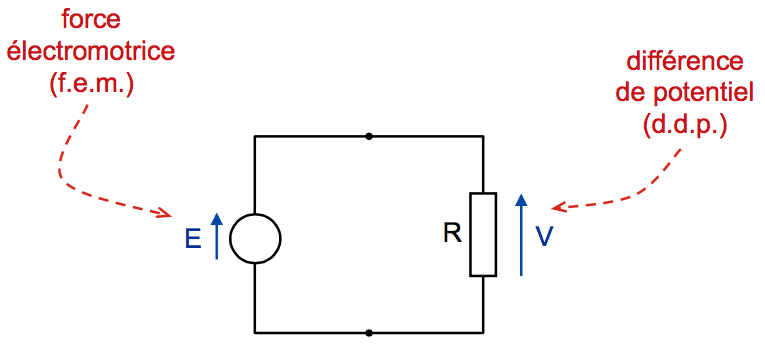
\includegraphics[width=0.6\textwidth]{fig/2_fem.png}
            \caption{Une force électromotrice}
            \label{fig:fem}
        \end{center}
    \end{figure}

    Convention de représentation de la ddp : la flèche de tension pointe vers le
    potentiel le plus positif.

    \subsubsection{Energie et puissance}

    \paragraph{Charge} La charge se mesure en \textcolor{red}{[C]}). Un électron
    porte une charge élémentaire négative notée $e$, qui vaut environ $-1,6.10^{-19}$C.

    \paragraph{Puissance} La puissance se mesure en \textcolor{red}{[W]}) et
    oscillera dans ce cours entre 10$\mu$W et 10W.

    \subsubsection{Energie et puissance}
    Formule de la puissance instantanée : $$ p(t) = v(t).i(t) $$

    \paragraph{Convention récepteur} Les flèches de courant et de tension sont
    de sens opposés

    \paragraph{Convention générateur} Les flèches de courant et de tension sont
    de même sens\\

    Dans les deux cas, $i>0$ et $v>0$.

    \paragraph{Dipôle passif} Un dipôle est \textit{passif} si il consomme de la puissance. On utilise alors la convention récepteur

    \paragraph{Dipôle actif} Un dipôle est \textit{actif} si il produit de la puissance. On utilise alors la convention générateur

    \subsubsection{Etat électrique, loi et caractéristique d'un dipôle}
    L'\textit{état électrique} d'un dipôle est le couple (I,V) de valeurs de
    courant et de tension qui s'appliquent à ce dipôle à un moment donné.

    \paragraph{Loi d'Ohm} $V = R.I$ (aussi appelée loi fondamentale d'un dipôle)

    \paragraph{Caractéristique} La \textit{caractéristique d'un dipôle} est le
    graphe représentant sa loi fondamentale dans le plan (I,V). Le point de fonctionnement
    du dipôle ne peut voyager que sur la caractéristique. \\
    \textbf{Exemple} : la caractéristique d'une source de tension idéale est une
    droite verticale (V constant).

    \paragraph{Résolution} On peut résoudre le circuit soit analytiquement, soit
    graphiquement (intersection des caractéristiques).

    \subsubsection{Principaux dipôles idéaux}
    \paragraph{Résistance} La résistance transforme la puissance électrique reçue
    en énergie thermique. Son unité est l'ohm \textcolor{red}{[$\Omega$]}, et
    oscillera dans ce cours entre $10\Omega$ et $10M\Omega$
    \begin{figure}[H]
        \begin{center}
            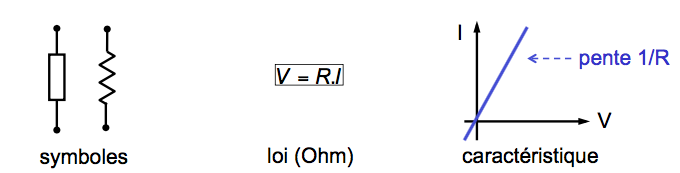
\includegraphics[width=0.6\textwidth]{fig/2_resistance.png}
            \caption{Dipôle résistance}
        \end{center}
    \end{figure}

    \paragraph{Source de tension} Ce dipôle fixe la tension.
    \begin{figure}[H]
        \begin{center}
            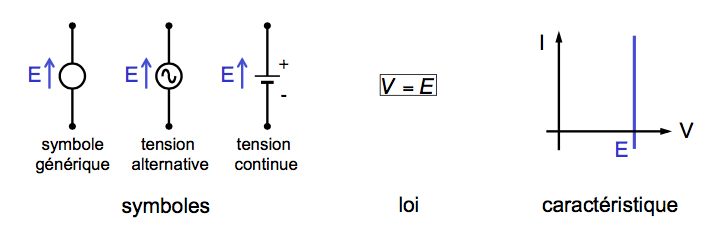
\includegraphics[width=0.6\textwidth]{fig/2_sourcetension.png}
            \caption{Source de tension}
        \end{center}
    \end{figure}

    \paragraph{Source de courant} Ce dipôle fixe le courant.
    \begin{figure}[H]
        \begin{center}
            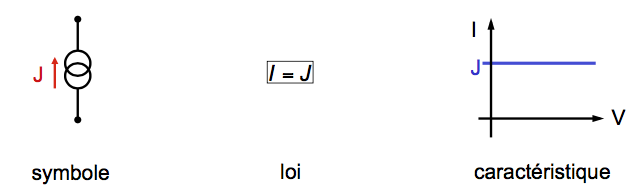
\includegraphics[width=0.6\textwidth]{fig/2_sourcecourant.png}
            \caption{Source de courant}
        \end{center}
    \end{figure}

    \paragraph{Court-circuit} Dipôle dans lequel la tension est nulle.
    \begin{figure}[H]
        \begin{center}
            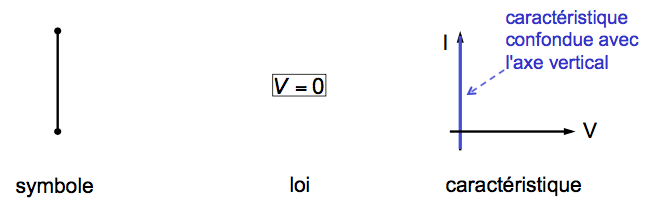
\includegraphics[width=0.6\textwidth]{fig/2_courtcircuit.png}
            \caption{Court-circuit}
        \end{center}
    \end{figure}

    \paragraph{Circuit ouvert} Dipôle dans lequel le courant est nul.
    \begin{figure}[H]
        \begin{center}
            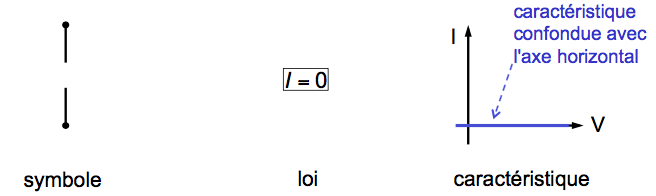
\includegraphics[width=0.6\textwidth]{fig/2_circuitouvert.png}
            \caption{Circuit ouvert}
        \end{center}
    \end{figure}

    \paragraph{Capacité} Sa caractéristique n'est pas représentable sur (I,V) car
    elle fait intervenir la notion de temps. Une capacité s'exprime en farads
    \textcolor{red}{[F]} et oscillera entre 10pF et 1mF.
    \begin{figure}[H]
        \begin{center}
            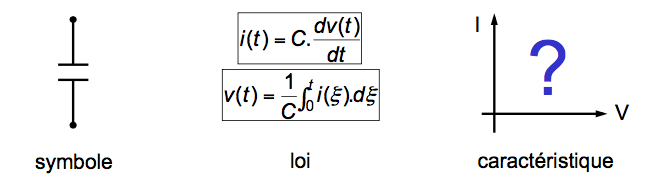
\includegraphics[width=0.6\textwidth]{fig/2_capacite.png}
            \caption{Capacité}
        \end{center}
    \end{figure}

    \paragraph{Inductance} Sa caractéristique n'est pas représentable sur (I,V) non plus.
    Les self-inductances sont exprimées en henris \textcolor{red}{[H]} et oscillent
    entre 10nH et 100mH.
    \begin{figure}[H]
        \begin{center}
            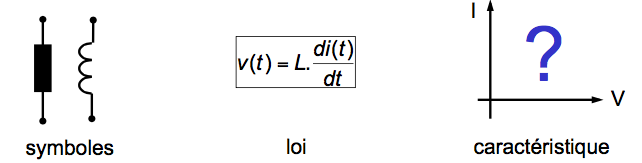
\includegraphics[width=0.6\textwidth]{fig/2_inductance.png}
            \caption{Capacité}
        \end{center}
    \end{figure}

    La capacité et l'inductance ont un statut particulier : elles ne dissipent
    pas de puissance mais sont capables d'emmagasiner de l'énergie et de la 
    restituer ensuite. Ces dipôles sont \textit{réactifs}.\\

    \`A un instant donné, l'énergie accumulée par ces composants vaut : 
    $E = \frac{C.V^2}{2}$ ou $E = \frac{L.I^2}{2}$\\

    \paragraph{Linéarité} On dit qu'un dipôle est \textit{linéaire} si sa caractéristique est une droite. Les systèmes linéaires bénéficient de propriétés particulières utiles. Les capacités et inductances sont considérées linéaires car elles peuvent s'exprimer linéairement en terme de charge électrique.
    $Q=C*V$
    $\phi=L*I$

    \subsection{Equivalent de Thévenin et adaptation d'impédance}

    \subsubsection{Equivalent de Thévenin d'une charge}
    Deux dipôles qui possèdent la même caractéristique sont dits \textit{équivalents}
    (au sens de Thévenin). 

    \paragraph{Exemple} Une résistance de $500\Omega$ et deux résistances de $250\Omega$
    en série.

    \paragraph{Résistance d'entrée} La \textit{résistance d'entrée $R_{in}$} de ce
    dipôle est :
    \begin{itemize}
        \item l'inverse de la pente de la caractéristique de ce dipôle
        \item la valeur de la résistance qui possède la même caractéristique que ce dipôle
    \end{itemize}

    On peut mesurer la résistance d'entrée d'une charge en lui appliquant une tension,
    en mesurant l'intensité du courant entrant dans le dipôle et en faisant
    le rapport entre la tension et le courant. ($R = \frac{V}{I} $)

    \subsubsection{Equivalent de Thévenin d'une source}
    Le problème avec les sources de tensions réelles, c'est que leur caractéristique
    n'est pas entièrement verticale. Leur tension réelle diminue en fait avec
    des intensités de courant plus grandes.\\

    Pour modéliser cette chute de tension, on rajoute une résistance en série
    avec la source de tension idéale. $$V = E - R_{out}.I$$
    \begin{figure}[H]
        \begin{center}
            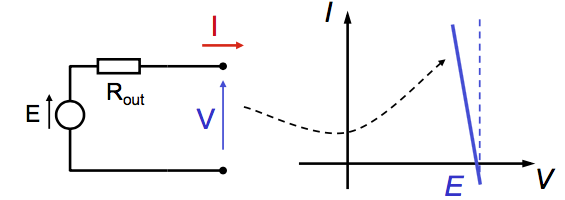
\includegraphics[width=0.6\textwidth]{fig/2_eqtheveninsource.png}
            \caption{Modélisation d'une source de tension réelle}
            \label{fig:2.2.2:eqtheveninsource}
        \end{center}
    \end{figure}

    L'ensemble résistance + source de tension est l'\textit{équivalent de Thévenin}
    de la source réelle. La résistance $R_{out}$ est appelée \textit{résistance
    de sortie}. Tout comme la résistance d'entrée d'une charge, elle est fictive.\\

    La ddp E (sur la fig \ref{fig:2.2.2:eqtheveninsource}) est appelée \textit{
    f.e.m. à vide} car V est égale à E uniquement lorsque la source n'est pas chargée.\\

    On mesure l'équivalent de Thévenin comme suit :
    \begin{itemize}
        \item mesure de la f.e.m. à vide (on place un voltmètre directement à la sortie de la source)
        \item détermination de la résistance de sortie (fig \ref{fig:2.2.2:mesurethevenin}).
    \end{itemize}

    \begin{figure}[H]
        \begin{center}
            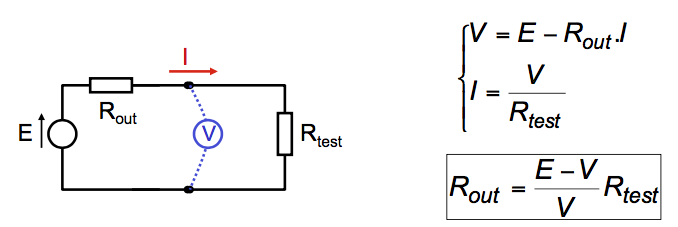
\includegraphics[width=0.6\textwidth]{fig/2_mesurethevenin.png}
            \caption{Détermination de la résistance de sortie}
            \label{fig:2.2.2:mesurethevenin}
        \end{center}
    \end{figure}

    Si $R{test}$ est un potentiomètre, on peut le régler de sorte que la tension
    V vaut la moitié de E $\Rightarrow R_{test} = R_{out}$

    \subsubsection{Théorèmes de Thévenin et de Norton}

    \paragraph{Théorème de Thévenin} Tout dipôle linéaire peut se modéliser
    sous la forme d'un équivalent de Thévenin, où l'équivalent de Thévenin
    est un circuit formé d'une f.e.m. placée en série avec une résistance.\\

    Note : la charge est un cas particulier où il n'y a pas de f.e.m.

    \begin{figure}[H]
        \begin{center}
            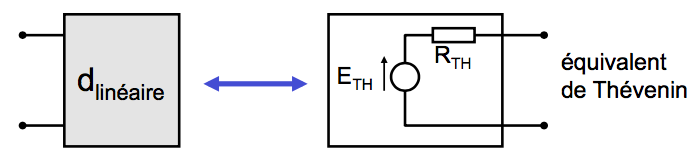
\includegraphics[width=0.6\textwidth]{fig/2_eqthevenin.png}
            \caption{Equivalent de Thévenin}
            \label{fig:2_eqthevenin}
        \end{center}
    \end{figure}

    \paragraph{Théorème de Norton} Tout dipôle linéaire peut se modéliser
    sous la forme d'un équivalent de Norton, où l'équivalent de Norton
    est un circuit formé d'une source de courant placée en parallèle avec une résistance.

    \begin{figure}[H]
        \begin{center}
            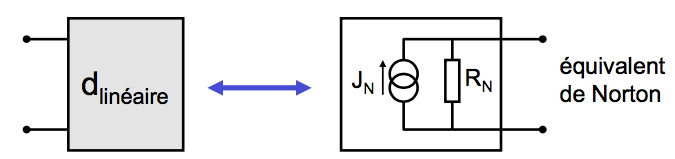
\includegraphics[width=0.6\textwidth]{fig/2_eqnorton.png}
            \caption{Equivalent de Norton}
            \label{fig:2_eqnorton}
        \end{center}
    \end{figure}

    \paragraph{Equivalences} On peut facilement passer de l'un à l'autre :
    \begin{align*}
        \begin{cases}
            R_{TH}&= R_N\\
            E_{TH}&= R_N . J_N
        \end{cases}
    \end{align*}

    \paragraph{Dipôles réactifs} Un dipôle réactif ne possède pas de caractéristique
    dans le plan (I,V). Ils possèdent cependant un équivalent de Thévenin (ou Norton).
    Il suffit de remplacer la résistance par une impédance.

    \paragraph{Dipôles non-linéaires} On va obtenir l'équivalent de Thévenin "à petits signaux".
    Il s'agit de l'équivalent de Thévenin de la tangente au point de fonctionnement.
    Cet équivalent n'est donc valable que pour de très faibles variations.

    \subsubsection{Equivalent de Thévenin d'un quadripôle}
    Voici le schéma de l'équivalent de Thévenin d'un quadripôle :
    \begin{figure}[H]
        \begin{center}
            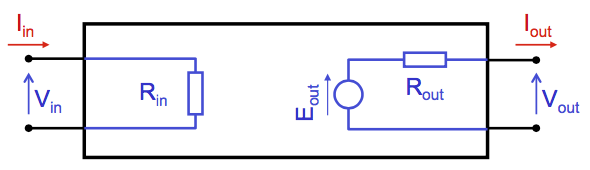
\includegraphics[width=0.6\textwidth]{fig/2_eqtheveninquad.png}
            \caption{Equivalent de Thévenin}
            \label{fig:2_eqtheveninquad}
        \end{center}
    \end{figure}
    On considère en fait l'entrée comme une charge et la sortie comme une source.
    Les conventions récepteur/générateur s'appliquent.

    \paragraph{Source commandée} Dans la fig \ref{fig:2_eqtheveninquad}, si le 
    quadripôle est un ampli, la tension de sortie doit logiquement être $A$ fois
    plus grande que la tension d'entrée. $V_{out}$ dépend de la tension d'entrée
    du quadripôle $V_{in}$ : $E_{out} = A . V_{in}$. Dans ce cas, $E_{out}$ est une 
    source de tension particulière dont la valeur dépend de la tension ou du courant
    en un autre endroit du montage : c'est une \textit{source commandée}.

    \subsubsection{Adaptation d'impédance: cas général}
    \paragraph{Adaptation d'impédance en tension} On considère un appareil amont
    délivrant un signal de tension à un appareil aval. Chacun des appareils
    peut être décrit par son équivalent de Thévenin. Voici comment on peut 
    calculer la tension entre les deux appareils (idée : diviseur résistif)

    \begin{figure}[H]
        \begin{center}
            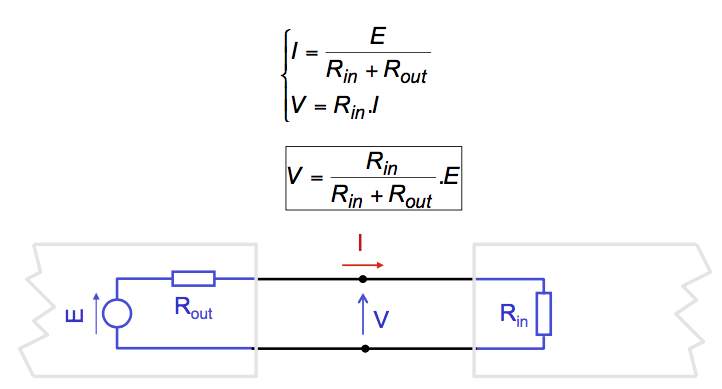
\includegraphics[width=0.6\textwidth]{fig/2_adaptimpedtension.png}
            \caption{Tension reçue par la charge}
            \label{fig:2_adaptimpedtension}
        \end{center}
    \end{figure}

    La tension est donc atténuée d'un facteur $\frac{R_{in}}{R_{in}+R_{out}}$. 
    Il faut donc avoir un $R_{in}$ très élevé ou un $R_{out}$ très faible
    pour limiter la dégradation.

    \paragraph{Critère d'adaptation en tension} Lorsqu'on transmet un signal
    de tension entre deux appareils, il faut une impédance d'entrée élevée
    et une impédance de sortie faible.

    \paragraph{Adaptation d'impédance en courant} Si l'appareil amont se comporte
    davantage comme une source de courant, on utilise l'équivalent de Norton.
    On calcule le courant reçu par l'appareil aval : 
    \begin{figure}[H]
        \begin{center}
            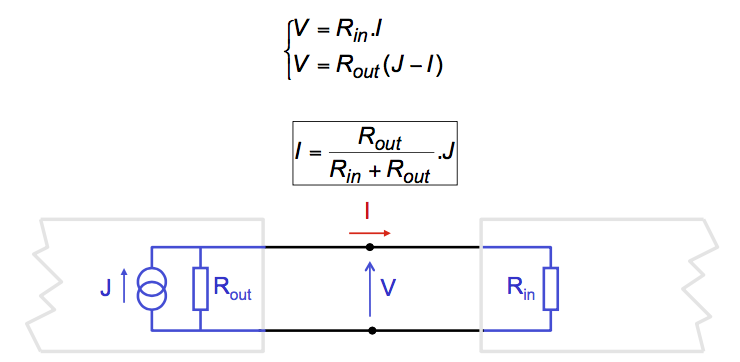
\includegraphics[width=0.6\textwidth]{fig/2_adaptimpedcourant.png}
            \caption{Courant reçu par la charge}
            \label{fig:2_adaptimpedcourant}
        \end{center}
    \end{figure}
    Le courant est effectivement atténué d'un facteur $\frac{R_{out}}{R_{out}+R_{in}}$.

    \paragraph{Critère d'adaptation en courant} Pour éviter une attéunation du courant
    transmis entre deux appareils, il faut une impédance d'entrée faible
    et une impédance de sortie élevée.

    \paragraph{Adaptation d'impédance en puissance}
    \begin{figure}[H]
        \begin{center}
            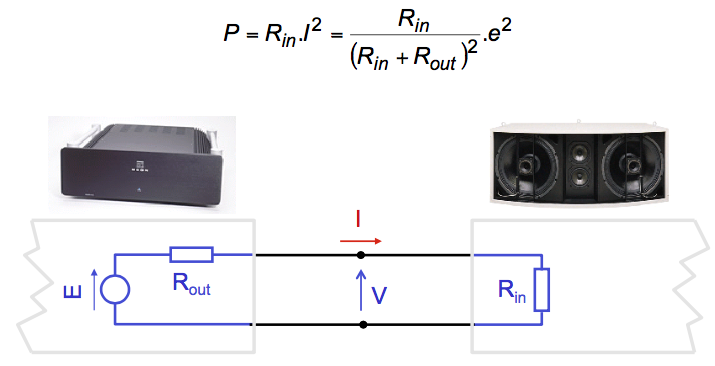
\includegraphics[width=0.6\textwidth]{fig/2_adaptimpedpuissance.png}
            \caption{Puissance reçue par la charge}
            \label{fig:2_adaptimpedpuissance}
        \end{center}
    \end{figure}

    \paragraph{Critère d'adaptation en puissance} On obtient un maximum de puissance
    transmise entre deux appareils lorsque les impédances sont égales. (remarque :
    ce maximum vaut \textbf{la moitié} de la puissance délivrée par l'appareil amont)

    \subsubsection{Application aux instruments de mesure}
    \paragraph{Voltmètre} Modélisé comme une charge, il doit avoir une
    impédance d'entrée beaucoup plus élevée que l'impédance existant entre les 
    noeuds utilisés pour faire la mesure.

    \paragraph{Ampèrementre} Critère classique d'adaptation d'impédance en courant:
    il doit avoir une impédance d'entrée beaucoup plus faible que l'impédance
    existant entre les noeuds utilisés pour faire la mesure.


    \subsection{Résoudre un schéma}
    \subsubsection{\'Etapes canoniques}
    \begin{enumerate}
        \setcounter{enumi}{-1}
        \item (boucler les boucles)
        \item définir les courants
        \item définir les tensions (ddps)
        \item écrire les équations de noeud (courants)
        \item écrire les équations de maille (tensions)
        \item écrire les lois des dipôles
        \item résoudre le système 3-4-5
        \item (parfaire la finition)
    \end{enumerate}

    \subsubsection{Théorème de superposition}
    \textbf{Valable uniquement pour les circuits linéaires!}\\

    Il faut supprimer toutes les sources sauf une. On remplace :
    \begin{itemize}
        \item les sources de tension par un court-circuit
        \item les sources de courant par un circuit ouvert
    \end{itemize}
    On peut ensuite sommer les contributions individuelles de chaque source.

    \paragraph{Exemple} Voici un exemple :
    \begin{figure}[H]
        \begin{center}
            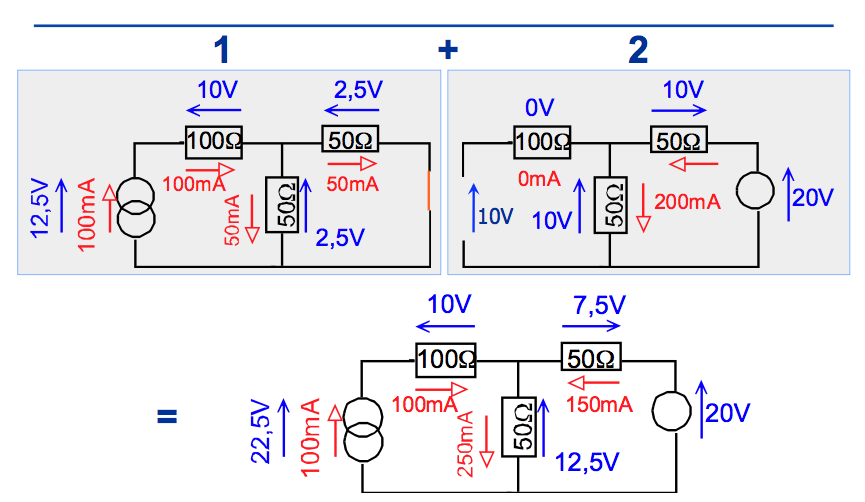
\includegraphics[width=0.7\textwidth]{fig/2_superposition.png}
            \caption{Application du principe de superposition}
            \label{fig:2_superposition}
        \end{center}
    \end{figure}

    \subsection{Composants réactifs}
        \begin{itemize}
            \item Les dipôles réactifs sont les capacités et inductances.
            \item Ne consomment pas de puissance
            \item Sont duals l'un de l'autre
            \item Deux aspects : temporel et fréquentiel
        \end{itemize}
        \subsubsection{Circuit RC en temporel}
            Lois fondamentales
            \begin{itemize}
                \item La DDP régit la charge/décharge
                \item Loi HF : la DDP ne varie pas instantanément
                \item Loi BF : $ t>> \rightarrow i = 0 $
            \end{itemize}

            En résolvant un circuit RC
            \begin{figure}[H]
                \begin{center}
                    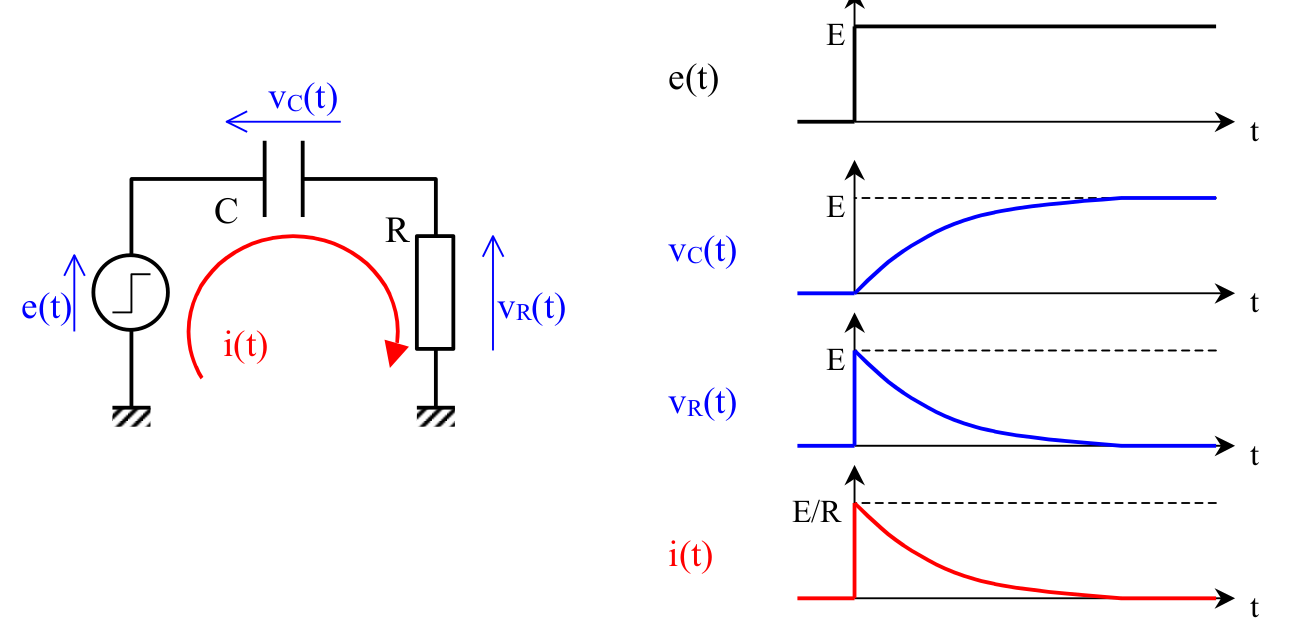
\includegraphics[width=0.7\textwidth]{fig/2_rc_temp2.png}
                    \caption{Circuit RC}
                    \label{fig:2_superposition}
                \end{center}
            \end{figure}
            On obtient la résolution analytique : 
            \begin{figure}[H]
                \begin{center}
                    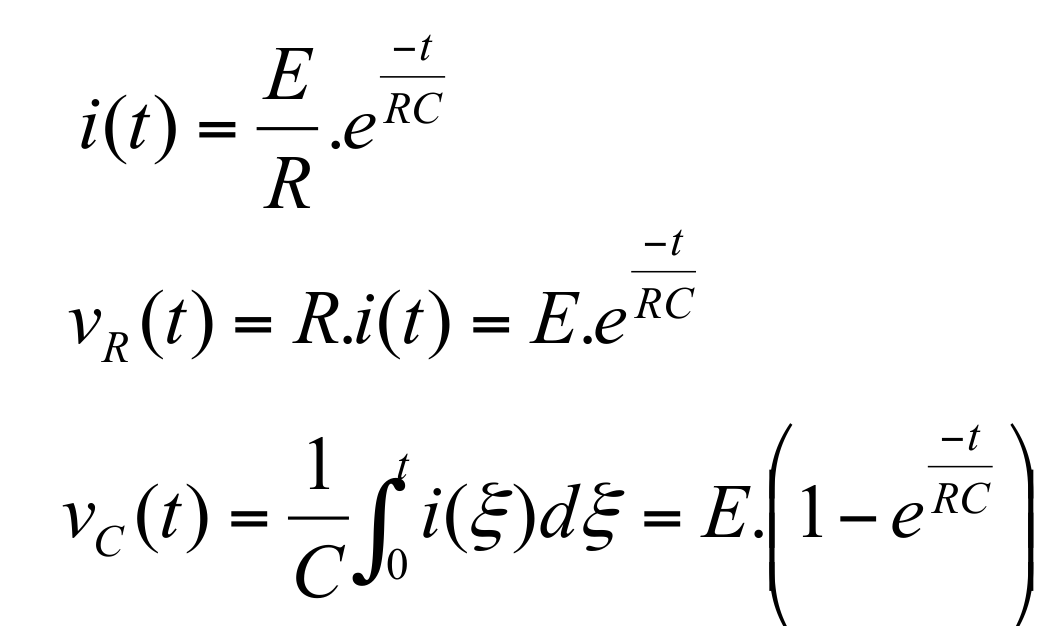
\includegraphics[width=0.7\textwidth]{fig/2_rc_temp.png}
                    \caption{Résolution analytique du circuit RC}
                    \label{fig:2_superposition}
                \end{center}
            \end{figure}
            Compliqué et long mais on peut simplifier en utilisant les lois fondamentales :  
            \begin{figure}[H]
                \begin{center}
                    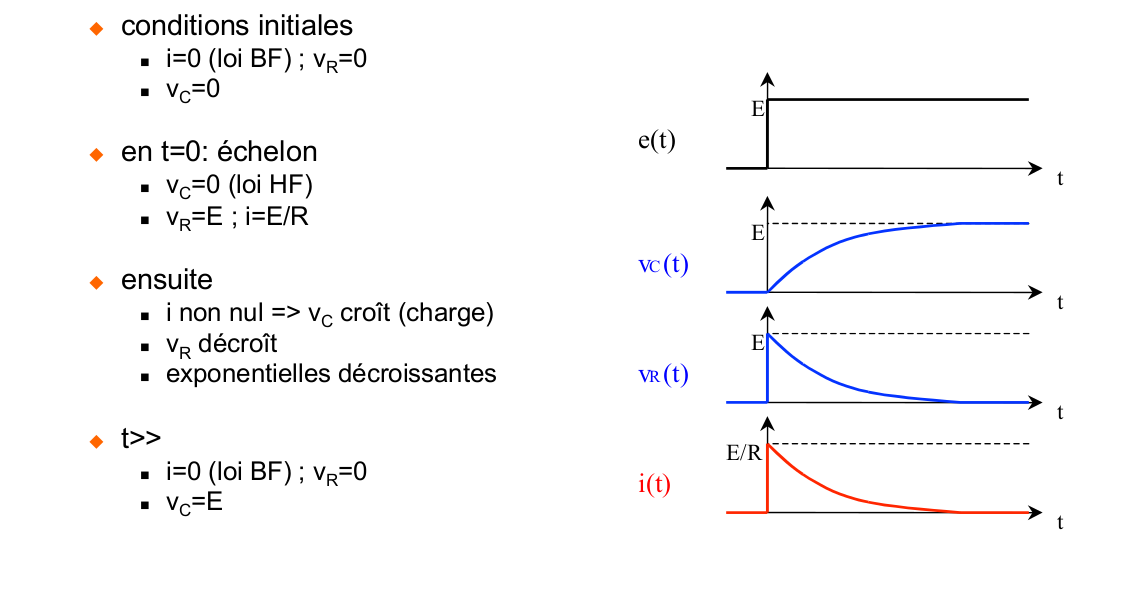
\includegraphics[width=0.7\textwidth]{fig/2_rc_temp3.png}
                    \caption{Résolution intuitive du circuit RC}
                    \label{fig:2_superposition}
                \end{center}
            \end{figure}
            \begin{itemize}
                \item La constante de temps de la charge/décharge de la capacité : $ \tau=R*C$
                \item 63\% après $ \tau $
                \item 95\% après $ 3*\tau $
                \item 99\% après $ 5*\tau $
                \item $ V_{C}(t) $ est un filtre passe-bas de $ e(t) $
                \item $ V_{R}(t) $ est un filtre passe-haut de $ e(t) $
                \item La fréquence de coupure : $ f_{0} = \frac{1}{2\pi\tau} $
                \item La pulsation de coupure : $ \omega_{0} = \frac{1}{\tau} $
            \end{itemize}
        \subsubsection{Circuit RL en temporel}
            Magnétisation : augmentation du courant. \\
            Démagnétisation : diminution du courant. \\
            Lois fondamentales
            \begin{itemize}
                \item Loi HF : le courant ne varie pas instantanément
                \item Loi BF : $ t>> \rightarrow v = 0 $
            \end{itemize}
            \begin{figure}[H]
                \begin{center}
                    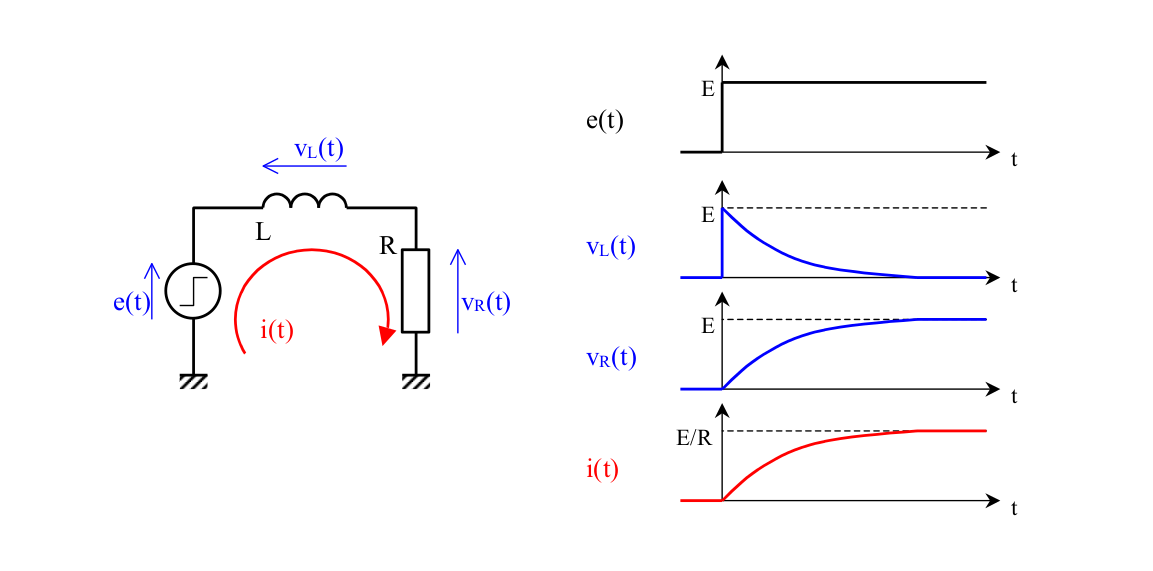
\includegraphics[width=0.7\textwidth]{fig/2_rl_temp.png}
                    \caption{Résolution intuitive du circuit RL}
                    \label{fig:2_superposition}
                \end{center}
            \end{figure}
            \begin{itemize}
                \item $ \tau = \frac{L}{R} $
                \item $ V_{L}(t) est un filtre passe-haut de e(t) $
                \item $ V_{R}(t) est un filtre passe-bas de e(t) $
                \item La fréquence et la pulsation de coupure sont les mêmes que RC
            \end{itemize}


\section{Amplificateurs opérationnels (Chapitre 4)}
    \subsection{Pourquoi amplifier}
        \begin{itemize}
            \item Signaux très faibles
            \item Régler le niveau logique
            \item Amplifier en amont d'un CAN/ADC (Convertisseur Analogique/Numérique)
        \end{itemize}

    \subsection{Propriétés de base}
        \subsubsection{Définitions}
            \begin{figure}[H]
                \begin{center}
                    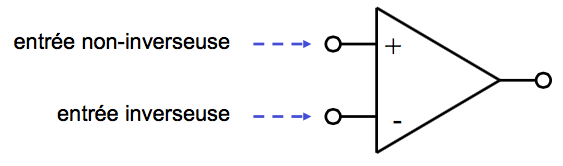
\includegraphics[width=0.6\textwidth]{fig/4_ampliop.png}
                    \caption{Ampli Op}
                \end{center}
            \end{figure}
            \begin{itemize} 
            \item C'est un circuit intégré à 8 pattes (deux bornes d'entrée et une borne de sortie). Il est considéré comme un quadripôle.
            \item L'entrée $-$ est l'entrée \textit{inverseuse}.
            \item L'entrée $+$ est l'entrée \textit{non-inverseuse}.
            \item Chacune des entrées et sortie reçoit un signal de tension mesuré par rapport à la masse. Ils sont notés respectivement $ V^{+} $, $ V^{-} $ et $ V_{out} $
            \item La \textit{tension d'entrée différentielle} est notée $ V_{d} = V^{+} - V^{-} $
            \item La fonction d'un ampli-op est d'amplifier cette tension
            \end{itemize}
        \subsubsection{Loi fondamentale et gain}
        La \textit{fonction d'amplification} d'un ampli-op est $ V_{out} = A*V_{d} $ \\
        Le \textit{gain} $A$ d'un ampli op est le facteur d'amplification entrée son entrée différentielle et sa sortie. \\
        \begin{itemize}
            \item $A$ est sans dimension.
            \item $A$ est très élevé (typiquement entre 30000 et 100000). On fait l'hypothèse qu'il est infini.
            \item $A$ n'a de sens que si la tension d'entrée est très faible.
            \item Les tensions $V_{d}$ et $V_{out}$ peuvent être aussi bien positives que négatives (par exemple dans le cas d'un courant alternatif)
        \end{itemize}

        \subsubsection{Bornes d'alimentation}
            \begin{figure}[H]
                \begin{center}
                    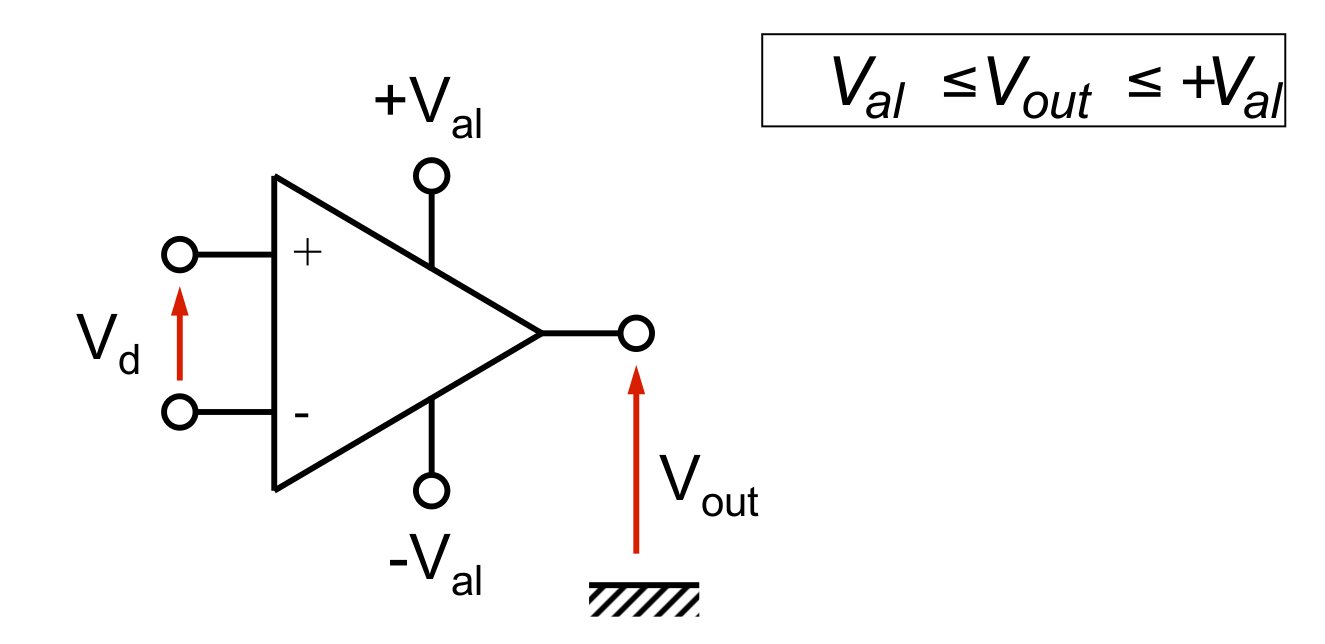
\includegraphics[width=0.6\textwidth]{fig/4_ampliop_alim.png}
                    \caption{Ampli Op}
                \end{center}
            \end{figure}
            Pour amplifier le signal, l'ampli-op a besoin d'une source d'énergie qui est fournie par des bornes d'alimentation.\\
            \begin{itemize}
                \item Elles sont le plus souvent symétriques
                \item Généralement $-12V$ et $+12V$ ou $-15V$ et $+15V$
                \item La tension de sortie ne peut pas sortir de la gamme fixée par ces tensions d'alimentation
            \end{itemize}
            L'ampli op est donc un composant \textbf{actif} car il ajoute de la puissance dans le circuit.
        \subsubsection{Ampli-Op réel : 741}
            \begin{figure}[H]
                \begin{center}
                    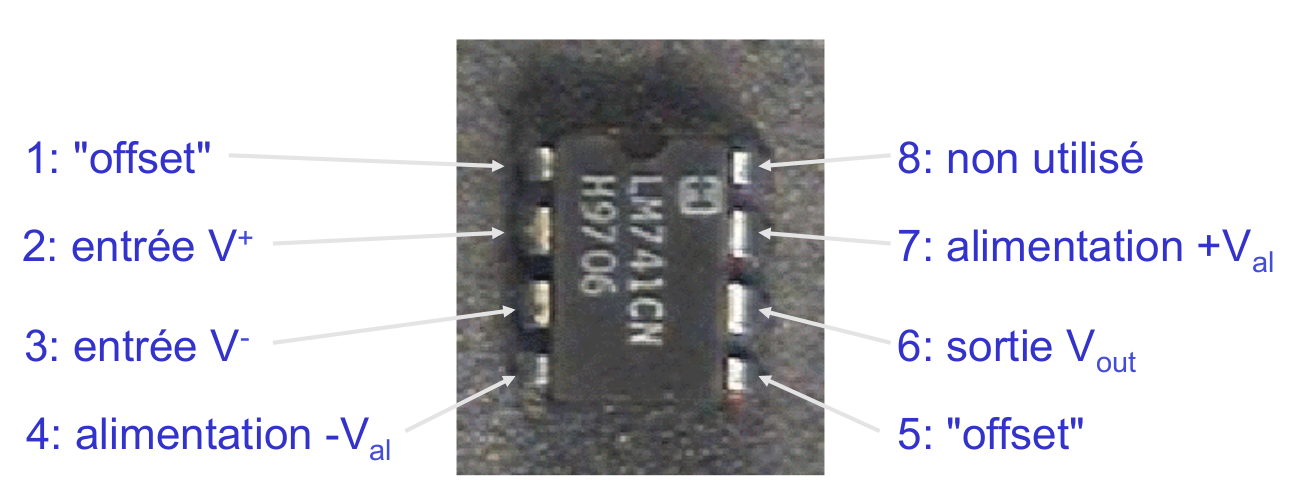
\includegraphics[width=0.6\textwidth]{fig/4_ampliop_reel.png}
                    \caption{Ampli Op}
                \end{center}
            \end{figure}

    \subsubsection{Impédances d'entrée et de sortie}
    Particularité : l'impédance d'entrée $Z_{in}$ d'un ampli-op est différentielle.
    Elle est très élevée, on fait même souvent l'approximation qu'elle est infinie.\\

    Inversement, l'impédance de sortie de l'ampli-op est très faible. On fait
    souvent l'approximation qu'elle est nulle.\\

    Pour être complets, il faut encore identifier la source commandée $E_{out}$
    de l'équivalent de Thévenin. On néglige la résistance de sortie, donc 
    $E_{out} = A.V_{in} = A.V_d$.

    \subsubsection{Caractéristique de transfert et principe du zéro virtuel}
    La \textit{caractéristique de transfert} d'un ampli-op est le rapport entre
    sa tension d'entrée et tension de sortie (fig) 

    \begin{figure}[H]
        \begin{center}
            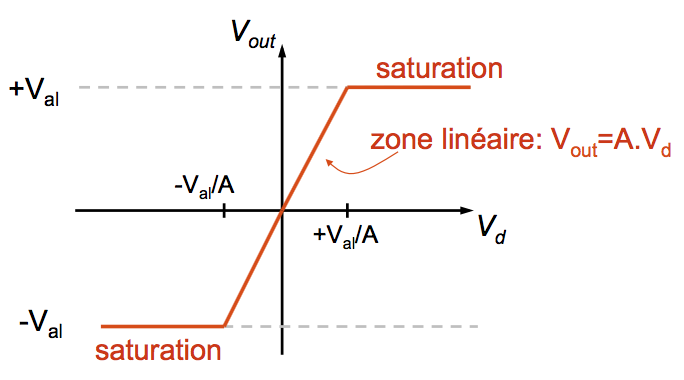
\includegraphics[width=0.6\textwidth]{fig/4_cartransfert.png}
            \caption{Caractéristique de transfert d'un ampli-op}
            \label{fig:4_cartransfert}
        \end{center}
    \end{figure}

    On y distingue trois zones
    \begin{itemize}
        \item la zone linéaire qui correspond à la loi fondamentale, très étroite
        (car le gain est très élevé)
        \item les zones de saturation là où la sortie atteint les tensions d'alimentation
    \end{itemize}

    \paragraph{Principe du zéro virtuel} Tant qu'un ampli-op ne sature pas, sa 
    tension différentielle est virtuellement nulle.\\

    On peut négliger $V_d$ \textbf{tant qu'on est dans la zone linéaire}. Cela
    revient à approximer $V^+ = V^-$.\\

    Le seul problème est alors qu'on approxime $V_d$ à zéro précisément au seul
    endroit où on a besoin de sa valeur. Le zéro virtuel consiste en fait à faire
    deux approximations simultanées, l'autre étant que A est infini.\\

    Dernière chose à retenir : pour amplifier un signal, un ampli-op seul, tel-quel
    est inutilisable car il sature très vite. Il faudra l'utiliser dans un montage.


    \subsection{Deux montages amplificateurs}
    \subsubsection{L'ampli non-inverseur (calcul classique)}

    Voici le schéma d'un montage amplificateur non-inverseur : 
    \begin{figure}[H]
        \begin{center}
            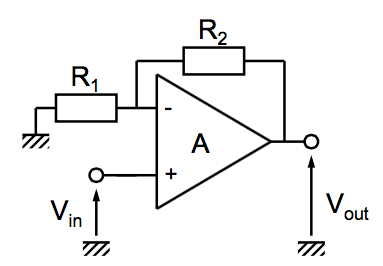
\includegraphics[width=0.4\textwidth]{fig/4_montampni.png}
            \caption{Montage amplificateur non-inverseur}
            \label{fig:4_montampni}
        \end{center}
    \end{figure}
    Attention, nous parlerons maintenant du montage, y compris quand on parle de gain.
    On voit aussi sur le montage que $R_2$ est en rétroaction.

    \paragraph{Calcul du gain $A_{non_inv}$}
    On peut noter $V_{out} = A.(V^+-V^-)$ et $V^+ = V_{in}$. Pour trouver $V^-$, 
    on remarque que $R_1$ et $R_2$ forment un diviseur résistif. Donc, 
    $V^- = \frac{R_1}{R_1+R_2}V_{out}$. (Cette relation n'est valable que
    sous l'hypothèse de l'impédance d'entrée infinie!).\\

    Avec ces 3 équations et l'hypothèse que A est très élevé, on peut arriver 
    à $A_{non-inv} \approx 1 + \frac{R_2}{R_1}$.\\

    Par exemple, pour amplifier 100 fois $V_{in}$, il suffit de prendre $R_1 = 1k\Omega$
    et $R_1 = 99k\Omega$

    \paragraph{Gain variable}
    On peut remplacer $R_2$ par un potentiomètre, mais le gain sera toujours de
    minimum 1.

    \paragraph{Impédance d'entrée du montage}
    On peut faire le raisonnement suivant :
    \begin{enumerate}
        \item $V_{in}$ est appliquée à l'entrée non-inverseuse de l'ampli-op
        \item comme l'impédance d'entrée de l'ampli-op est infinie, aucun courant
        ne peut rentrer par cette borne $\Rightarrow I_{in} = 0$
        \item l'impédance d'entrée dun montage est donc elle-même infinie.
    \end{enumerate}


    \subsubsection{L'ampli inverseur (calcul classique)}
    Son schéma est quasiment identique :
    \begin{figure}[H]
        \begin{center}
            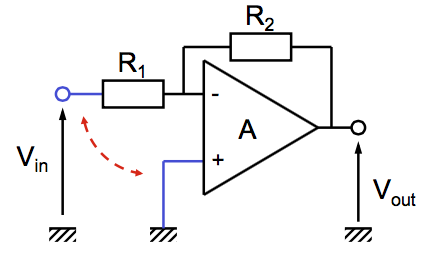
\includegraphics[width=0.4\textwidth]{fig/4_montampi.png}
            \caption{Montage amplificateur inverseur}
            \label{fig:4_montampi}
        \end{center}
    \end{figure}
    On peut calculer son gain et obtenir $A_{inv} \approx - \frac{R_2}{R_1}$. On 
    note qu'il est négatif et qu'on peut, lui, entièrement l'annuler.

    \paragraph{Impédance}
    Le courant $I_{in}$ n'est autre que le courant circulant dans $R_1$ et aussi
    dans $R_2$ (puisque l'impédance d'entrée de l'ampli-op est infinie). L'impédance est :
    $$ Z_{in} = \frac{V_{in}}{I_{in}}$$
    On peut donc écrire que ce courant vaut : $I_{in} = \frac{V_{in} - V_{out}}{R_1+R_2} $.
    Aussi, $V_{out} = A_{inv}.V_{in} = -\frac{R_2}{R_1}.V_{in} $.\\

    Conclusion : l'impédance d'entrée du montage inverseur vaut $R_1$, ce qui est
    très faible.

    \subsubsection{Calcul rapide avec le principe du zéro virtuel}
    On peut approximer que $V^+ = V^-$. Concernant le montage, on peut dire que
    $V^- = \frac{R_1}{R_1+R_2}V_{out}$. Si on égalise ces deux équations, on trouve
    immédiatement le gain du montage : 
    $$ A_{non-inv} = \frac{V_{out}}{V_{in}} = 1 + \frac{R_2}{R_1} $$

    \subsubsection{Analyse de la rétroaction}
    En gros, dans le montage non-inverseur, quand on applique 10mV à $V^+$, 
    $V_{out}$ ne montera pas directement à 30000 fois la valeur de $V_{in}$.
    Cette valeur montera graduellement. Or, plus elle monte, plus la valeur 
    sur $V^-$ monte. $V_d$ diminue donc, et $V_{out}$ ne doit plus monter
    si haut. Il y a un moment où les deux valeurs s'équilibrent.\\

    En fait, le fait que $R_2$ soit rétroactive permet que $V^-$ "poursuive" $V^+$.
    C'est elle qui assure le zéro virtuel.

\section{Les diodes (chapitre 5)}
    
    \subsection{Introduction}
    La diode est le semi-conducteur le plus simple. Sa première fonction de base est de 
    redresser une tension (= convertir une grandeur alternative en grandeur positive).
    Le redressement est également utilisé pour démoduler des signaux.\\

    La deuxième fonction de base d'une diode est de limiter la tension (écrêtage).\\

    Les diodes sont également très présentes sous forme de LEDs.

    \subsection{La diode à jonction PN (idéale)}
    La diode a deux bornes, anode et cathode :
    \begin{figure}[H]
        \begin{center}
            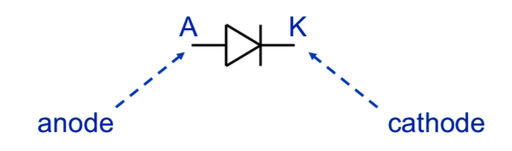
\includegraphics[width=0.4\textwidth]{fig/5_diode.png}
            \caption{Une diode}
            \label{fig:5_diode}
        \end{center}
    \end{figure}

    (De manière générale, le terme "cathode" désigne une borne qui "émet" des électrons
    et le terme "anode" désigne une borne qui capte des électrons).\\

    La diode est un composant passif qui n'admet de courant que dans le sens A$\rightarrow$K.\\

    Une diode idéale ne possède que deux états : passante et bloquante. Sa 
    caractéristique est donc en angle droit.
    \begin{figure}[H]
        \begin{center}
            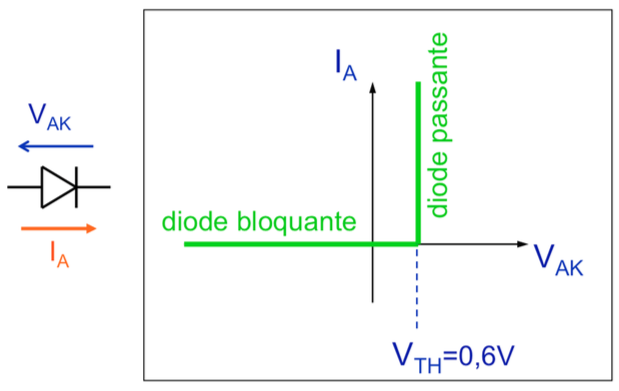
\includegraphics[width=0.5\textwidth]{fig/5_diodecar.png}
            \caption{Caractéristique d'une diode}
            \label{fig:5_diodecar}
        \end{center}
    \end{figure}
    La valeur $V_{TH}$ est la tension de seuil de la diode. Dans la plupart des cas,
    on peut considérer (pour les diodes PN) qu'elle vaut 0.6V.

    \paragraph{Diode passante}
    Lorsque la diode est passante, on peut dire que :
    \begin{align*}
        \begin{cases}
            V_{AK} &= V_{TH} = 0.6V\\
            I_A &> 0
        \end{cases}
    \end{align*}

    On se rend compte qu'une diode \textbf{passante} peut être assimilée à une
    source de tension idéale de valeur $V_{TH}$. Effectivement:
    \begin{itemize}
        \item sa caractéristique est une droite verticale
        \item elle impose une ddp à ses bornes mais pas le courant
    \end{itemize}
    La seule différence et qu'une source de tension admet un courant négatif, pas la diode.\\

    On peut même aller plus loin si toutes les tensions présentes dans le circuit
    sont nettement supérieures à 0.6V et considérer la diode comme un court-circuit.

    \paragraph{Diode bloquante}
    Quand elle est bloquante, on peut dire d'une diode que :
    \begin{align*}
        \begin{cases}
            V_{AK} &< V_{TH} = 0.6V\\
            I_A &= 0
        \end{cases}
    \end{align*}
    Une diode bloquante peut être assimilée à un circuit ouvert.

    \paragraph{Non-linéarité} La diode est un composant \textbf{non-linéaire}.
    On ne peut donc \textbf{pas appliquer le principe de superposition!}

    \subsection{Résoudre un circuit à diode}
    Tentons de résoudre le circuit suivant :
    \begin{figure}[H]
        \begin{center}
            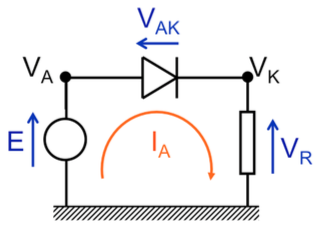
\includegraphics[width=0.4\textwidth]{fig/5_circuitdiode.png}
            \caption{Un circuit avec une diode}
            \label{fig:5_circuitdiode}
        \end{center}
    \end{figure}
    Il y a 3 inconnues : $V_{AK}, V_R$ et $I_A$. Il faut donc 3 équations :
    \begin{itemize}
        \item $E = V_{AK}+V_R$ (loi des mailles)
        \item $V_R = R.I_A$
        \item la troisième relation devrait être la loi de la diode. Or il y en a 
        deux suivant que la diode est passante ou bloquante. Pour savoir laquelle
        prendre, il faut connaître l'état du circuit, mais pour connaître l'état
        du circuit, il faut connaître l'état de la diode...
    \end{itemize}

    Il faut donc utiliser un raisonnement par hypothèse :
    \begin{enumerate}
        \item poser une hypothèse
        \item raisonner comme si cette hypothèse était exacte
        \item vérifier si le résultat obtenu est compatible avec l'hypothèse
    \end{enumerate}

    Voici donc la procédure à suivre :
    \begin{enumerate}
        \item pour chaque diode, il n'y a que deux hypothèses : soit bloquante soit passante
        \item une fois l'état fixé par hypothèse, on impose la loi correspondante (l'égalité, 
        donc soit $V_{AK} = 0.6V$ soit $I_A=0$). On peut remplacer la diode
        dans le circuit par soit une source de tension (diode passante), soit
        un circuit ouvert (diode bloquante) pour faciliter la résolution.
        \item une fois le circuit résolu, il faut vérifier la compatibilité
        du résultat obtenu avec l'hypothèse. En particulier, il faut vérifier si :
        \begin{itemize}
            \item $I_A >0$ si on a choisi l'hypothèse d'une diode passante
            \item $V_{AK} < 0.6V$ si on a choisi l'hypothèse d'une diode bloquante
        \end{itemize}
    \end{enumerate}

    Voici un exemple de ce raisonnement :
    \begin{figure}[H]
        \begin{center}
            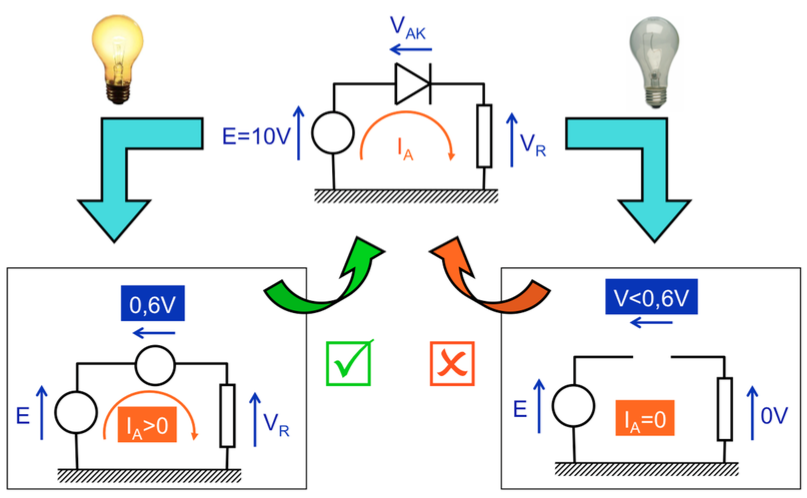
\includegraphics[width=0.5\textwidth]{fig/5_circuitdiodeexemple.png}
            \caption{Exemple de résolution d'un circuit à diodes}
            \label{fig:5_circuitdiodeexemple}
        \end{center}
    \end{figure}

    Dans l'exemple ci-dessus, E est fixé. S'il ne l'est pas, on applique le 
    même raisonnement mais on rajoute à notre réponse une condition (si E
    n'est pas fixé, la condition sera par exemple $E > V_{TH}$ ou $E < V_{TH}$).\\

    Une résolution graphique est aussi possible :
    \begin{figure}[H]
        \begin{center}
            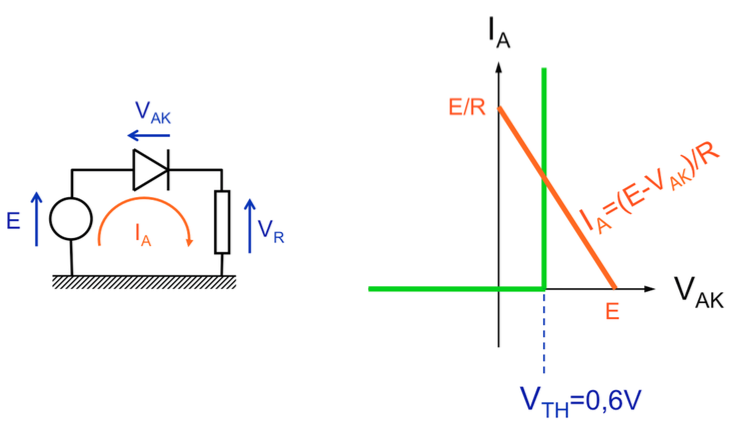
\includegraphics[width=0.5\textwidth]{fig/5_diodecircuitexemplegraphique.png}
            \caption{Exemple de résolution graphique d'un circuit à diodes}
            \label{fig:5_diodecircuitexemplegraphique}
        \end{center}
    \end{figure}

    \subsection{Diodes et polarisation}
    Nous allons voir comment polariser (= mettre de manière contrôlée à l'état passant ou bloquant) une diode.

    \begin{figure}[H]
        \begin{center}
            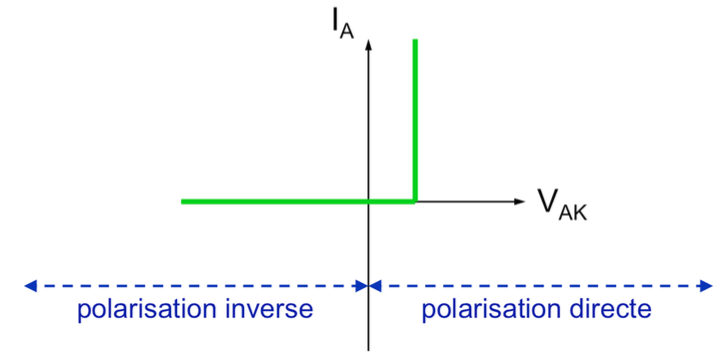
\includegraphics[width=0.5\textwidth]{fig/5_diodepolarisation.png}
            \caption{Polarisation d'une diode}
            \label{fig:5_diodepolarisation}
        \end{center}
    \end{figure}
    \begin{itemize}
        \item si $V_{AK} > 0$, la diode est dite en polarisation directe
        \item si $V_{AK} < 0$, la diode est dite en polarisation inverse
    \end{itemize}

    \paragraph{Rendre une diode bloquante}
    Il ne faut ... rien faire. On peut lui appliquer une tension jusqu'à $V_{TH}$.

    \paragraph{Rendre une diode passante}
    Il ne faut \textbf{jamais} lui appliquer directement une f.e.m.! Sinon, 
    le courant est indéterminé (fig \ref{fig:5_diodefem}), théoriquement infini.
    \begin{figure}[H]
        \begin{center}
            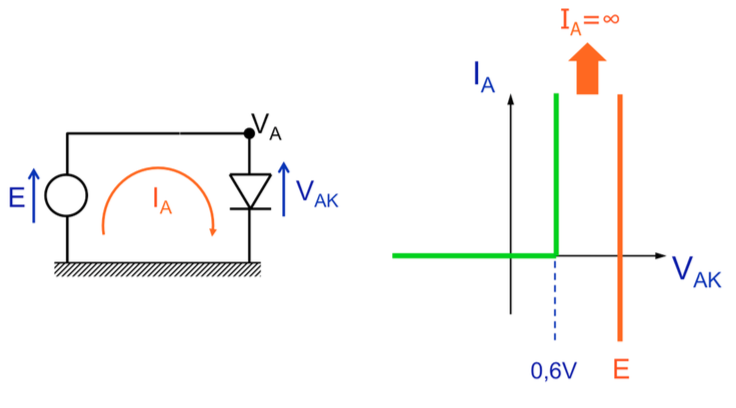
\includegraphics[width=0.5\textwidth]{fig/5_diodefem.png}
            \caption{\`A ne jamais faire}
            \label{fig:5_diodefem}
        \end{center}
    \end{figure}

    Il faut ajouter une résistance de limitation de courant :
    \begin{figure}[H]
        \begin{center}
            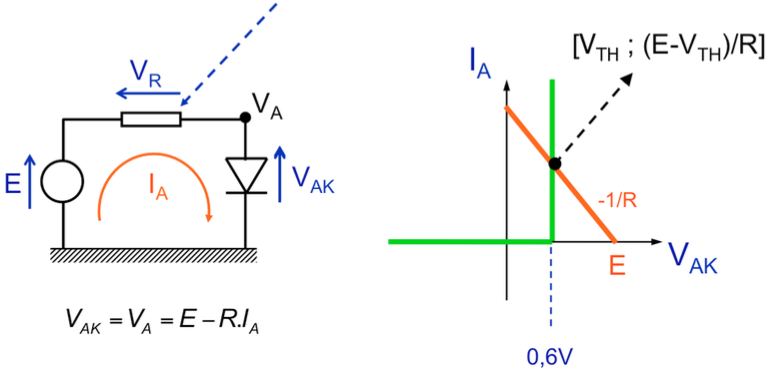
\includegraphics[width=0.5\textwidth]{fig/5_resistancelimitation.png}
            \caption{Résistance de limitation de courant}
            \label{fig:5_resistancelimitation}
        \end{center}
    \end{figure}
    On retombe alors sur le schéma simple redresseur, avec :
    \begin{align*}
        \begin{cases}
            V_{AK} &= V_{TH}\\
            I &=\frac{E-V_{TH}}{R}
        \end{cases}
    \end{align*}

    On peut aussi, plus simplement, utiliser une source de courant. Dans ce cas, 
    la diode fixe la ddp et la source fixe l'intensité du courant.

    \subsection{Principaux circuits à diodes}
    Dans les circuits suivants, on considère qu'on utilise des diodes idéales.

    \subsubsection{Redresseur simple alternance}
    \begin{figure}[H]
        \begin{center}
            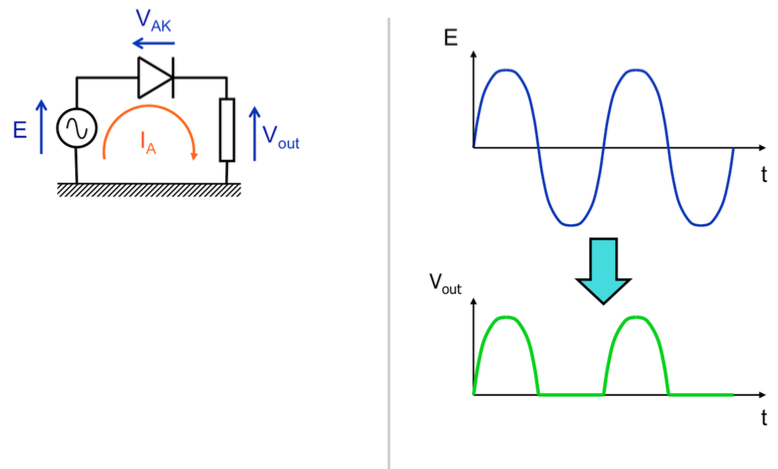
\includegraphics[width=0.6\textwidth]{fig/5_redresseursa.png}
            \caption{Redresseur simple alternance}
            \label{fig:5_redresseursa}
        \end{center}
    \end{figure}
    Ce circuit est appelé redresseur car une tension alternative (E) est transformée
    en tension uniquement positive($V_{out}$).\\

    Cette fonction de redressement est une des fonctions fondamentales de l'électronique.
    Elle est notamment utilisée :
    \begin{itemize}
        \item pour démoduler des signaux radios (en modulation AM)
        \item dans les alimentations pour transformer une tension alternative en
        tension continue.
    \end{itemize}

    Le redressement est indispensable dans les alimentations AC/DC. La fig \ref{fig:5_redressementalim} 
    montre les différentes étapes qu'une alimentation effectue pour assurer un 
    courant continu de 5V aux composants en aval. Ce principe n'est par contre
    plus très utilisé, on utilise maintenant plutôt des alimentations "à découpage", 
    vues plus tard.
    \begin{figure}[H]
        \begin{center}
            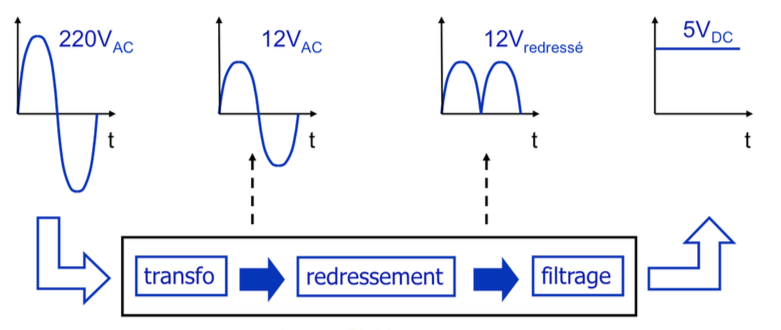
\includegraphics[width=0.6\textwidth]{fig/5_redressementalim.png}
            \caption{Exemple de fonctionnement d'une alimentation AC/DC}
            \label{fig:5_redressementalim}
        \end{center}
    \end{figure}

    \subsubsection{Sélecteur de maximum}
    La figure suivante est un sélecteur de maximum :
    \begin{figure}[H]
        \begin{center}
            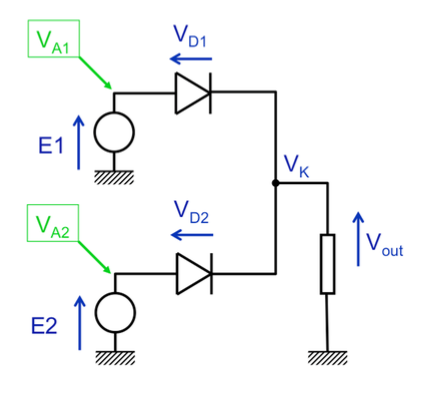
\includegraphics[width=0.4\textwidth]{fig/5_maxselector.png}
            \caption{Schéma d'un sélecteur de maximum}
            \label{fig:5_maxselector}
        \end{center}
    \end{figure}

    Faisons l'hypothèse que E1 > E2 > 0.
    Il y a quatre possibilités de résolutions pour le schéma ci-dessus.

    \begin{itemize}
        \item Supposons que D1 est \textbf{passante}. Dans ce cas, $V_K$ = E1-0,6V
        \begin{itemize}
            \item Supposons que D2 est \textbf{passante} aussi. Dans ce cas, $V_K$ devrait
            valoir E2-0,6V, ce qui est impossible. cette situation est donc impossible.
            \item Supposons que D2 est \textbf{bloquante}. Dans ce cas, on peut
            rempacer D2 par un circuit ouvert, ce qui coupe E2 du circuit. On 
            retombe dans le circuit simple redresseur.
        \end{itemize}
        \item Supposons que D1 est \textbf{bloquante}.
        \begin{itemize}
            \item Supposons que D2 est \textbf{passante}: $V_K$ = E2-$V_{TH}$. 
            D2 peut être passante, par contre la ddp sur D1 vaut 10V-(6V-0,06V) = 3,4V,
            ce qui contredit l'hypothèse D1 bloquante.
            \item, Si D2 est \textbf{bloquante}, on en arrive à la même situation
            que supra.
        \end{itemize}
    \end{itemize}
    En conclusion, on peut alculer que $V_{out}$ réplique la plus grande des deux
    tensions. Ce circuit est un sélecteur de maximum.\\

    NB. si E1 et E2 sont négatives, la masse est la plus grande des tensions, 
    $V_{out}$ vaut 0V.

    \subsubsection{Redresseur double alternance}
    \begin{figure}[H]
        \begin{center}
            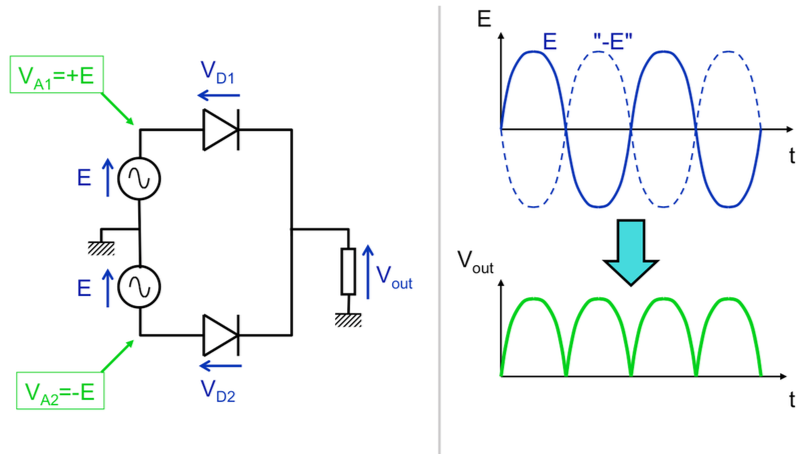
\includegraphics[width=0.6\textwidth]{fig/5_redresseurda.png}
            \caption{Redresseur double alternance}
            \label{fig:5_redresseurda}
        \end{center}
    \end{figure}
    C'est en fait un sélecteur de maximum alimenté par deux sources opposées.

    \subsubsection{Redresseur double alternance (2) : pont à 4 diodes}
    \begin{figure}[H]
        \begin{center}
            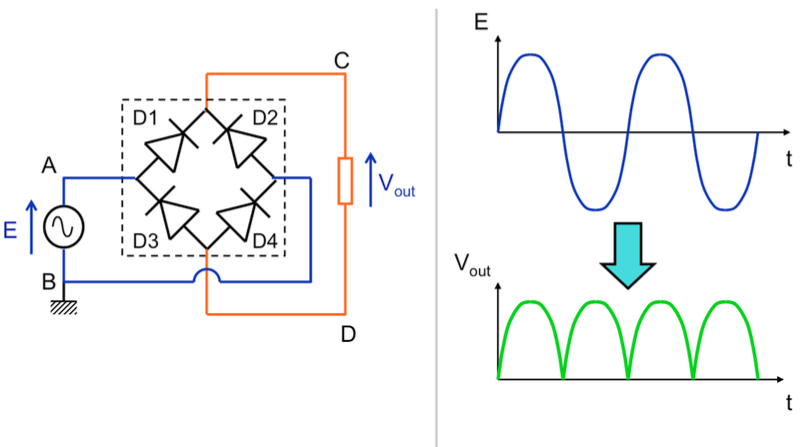
\includegraphics[width=0.6\textwidth]{fig/5_redresseurdapont.png}
            \caption{Redresseur double alternance (2) : pont à 4 diodes}
            \label{fig:5_redresseurdapont}
        \end{center}
    \end{figure}

    % TODO explication à écrire
    Explication à écrire. Je pense comprendre que D est à la masse mais pas sûr.

    \subsubsection{Limiteur de tension (écrêteur)}
    \begin{figure}[H]
        \begin{center}
            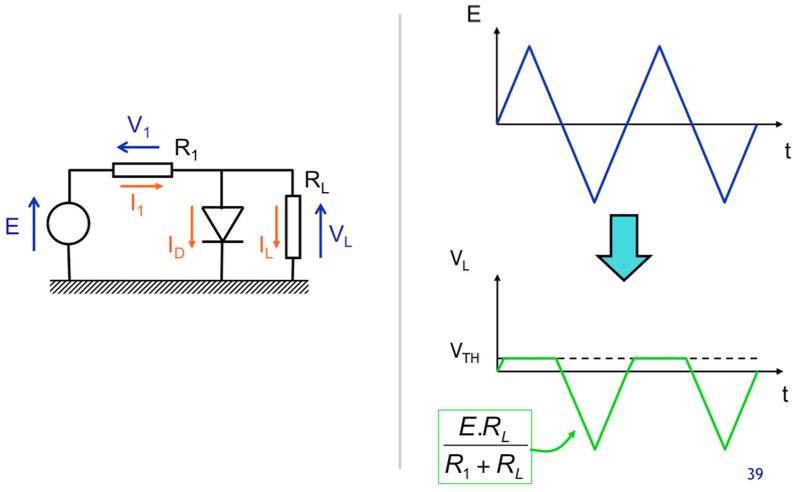
\includegraphics[width=0.6\textwidth]{fig/5_ecreteur.png}
            \caption{\'Ecrêteur}
            \label{fig:5_ecreteur}
        \end{center}
    \end{figure}
    En raisonnant par hypothèses, on voit que la tension à l'entrée de la diode
    ne peut dépasser $V_{TH}$. 

    \subsubsection{\'Ecrêteur polarisé}
    \begin{figure}[H]
        \begin{center}
            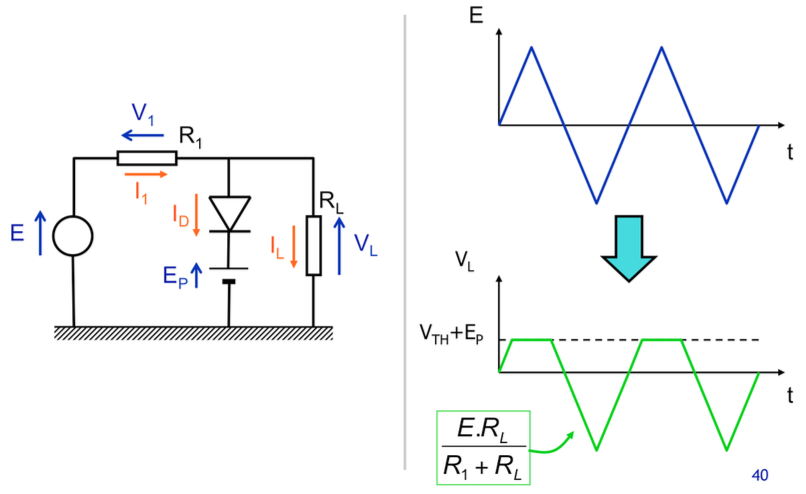
\includegraphics[width=0.6\textwidth]{fig/5_ecreteurpolarise.png}
            \caption{\'Ecrêteur polarisé}
            \label{fig:5_ecreteurpolarise}
        \end{center}
    \end{figure}
    Dans le montage précédent, la tension maximale est forcément $V_{TH}$. Ici,
    on rajoute une source de tension continue en série avec la diode. 
    La valeur à laquelle a lieu l'écrêtage n'est plus $V_{TH}$ mais $V_{TH} + E_p$\\

    Remarque : on retrouve ici la notion de polarisation qui consiste à ajuster
    le point de fonctionnement du montage au moyen d'une source continue. 

    \subsubsection{Détecteur de crêtes}
    \begin{figure}[H]
        \begin{center}
            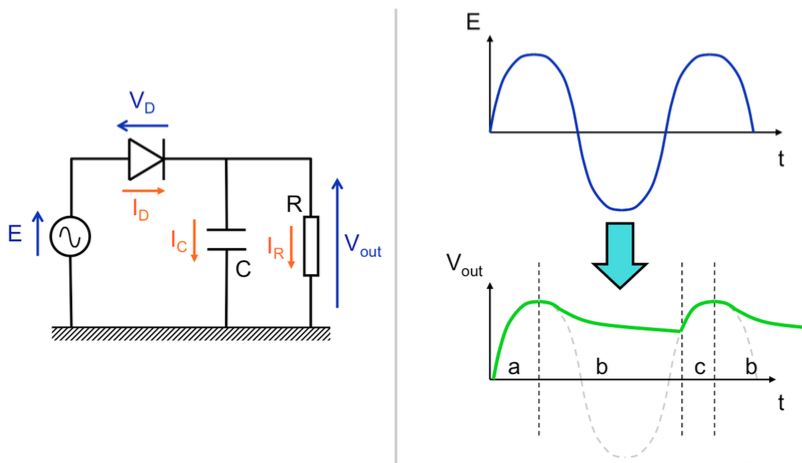
\includegraphics[width=0.6\textwidth]{fig/5_detecteurcretes.png}
            \caption{Détecteur de crêtes}
            \label{fig:5_detecteurcretes}
        \end{center}
    \end{figure}
    Ce circuit peut être vu comme une variante du redresseur simple alternance 
    où on place une capacité en parallèle sur la résistance de charge. Le circuit
    doit être dimensionné de telle sorte que la constante de temps du RC de sortie
    soit beaucoup plus grande que la période ou la durée d'une impulsion du signal d'entrée.
    \begin{itemize}
        \item \textbf{phase a :} la diode devient passante et le condensateur
        se charge à travers celle-ci
        \item \textbf{phase b :} la capa se décharge par la résistance (puisque
        la diode ne laissera pas passer le courant)
    \end{itemize}
    Note : le détecteur de crête sert notamment à 
    \begin{itemize}
        \item mesurer la valeur de crête d'un signal sans être synchronisé sur celui-ci
        \item détecter des impulsions très courte (capa = mémoire)
        \item la démodulation d'une porteuse modulée en amplitude (radio AM); on 
        choisit la constante de temps RC grande devant la période de porteuse, mais
        faible devant celle de la modulante. (fig \ref{fig:5_demod})
    \end{itemize}

    \begin{figure}[H]
        \begin{center}
            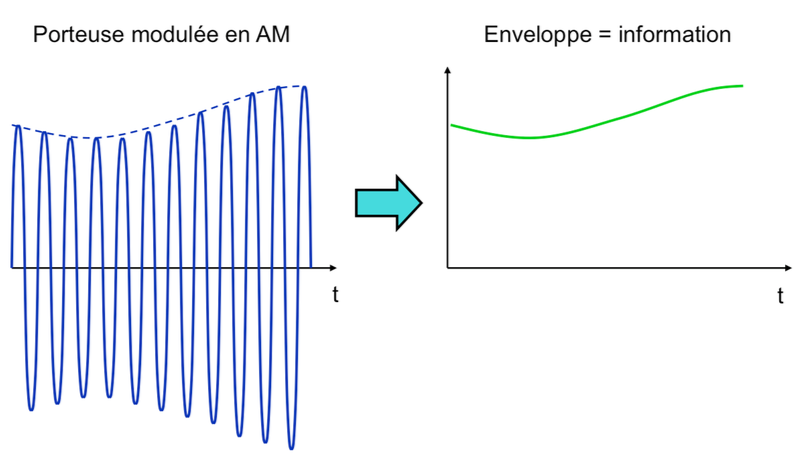
\includegraphics[width=0.6\textwidth]{fig/5_demod.png}
            \caption{Démodulation}
            \label{fig:5_demod}
        \end{center}
    \end{figure}

    La sinusoïde ne fait que transporter l'information, son enveloppe est la
    réelle information.
\end{document}
